\chapter{Realization}

The realization of the project can be separated into three distinct parts: \textbf{creating wall model}, \textbf{creating hold models}, \textbf{editor implementation}.
Each of the respective parts are open-source projects on GitHub, licensed under GPLv3:
\begin{itemize}
	\item \raisebox{-0.08em}{\includesvg[height=\baselineskip]{images/clis.svg}} -- the climber's scanner \footnote{\url{https://github.com/Climber-Apps/Clis}}
	\item \raisebox{-0.08em}{\includesvg[height=\baselineskip]{images/cled.svg}} -- the climber's editor \footnote{\url{https://github.com/Climber-Apps/Cled}}
\end{itemize}

\section{Creating wall model}
The wall model (figure \ref{fig:model}) has been created semi-automatically.
First, a set of 188 images was used by the Agisoft Metashape software to create a reference model.
This model was then manually edited in Blender 3D to remove possible modelling errors.
Since the wall consists only of straight segments connected together, this can be done relatively easily.
After manual changes, the resulting model was reimported to Metashape to generate the texture from the photos.

\begin{figure}
	\centering
	\includegraphics[width=\columnwidth]{images/wall/image.png}
	\caption{The model of the Smíchoff wall, created using Metashape and Blender.}
	\label{fig:model}
\end{figure}


\section{Creating hold models}
Since a regular climbing wall contains hundreds or even thousands of holds of varying sizes, it would be infeasible to model each of them manually.
It is important to automize as many steps as possible so that the amount of manual work done is minimized.

This has been acomplished using a turntable-based workflow, upon which the holds are placed and scanned.
The turntable turns the hold around for a stationary camera to take photos, which are then fed into the Agisoft Metashape protogrammetry software (+ Blender for post-processing) to generate the model.

The resulting workflow can process a single hold in $\sim 40$ seconds of scanning (taking $12$ photos, varies depending on lighting conditions), plus  $\sim4$ minutes of processing.

\subsection{Turntable design}
A three stepper-motor turntable has been developed and 3D printed using the Fusion 360 CAD software and an Ender Pro 5 3D printer \label{ref:turntable}.
An Arduino board and A4988 motor controllers are used for fine motor control (figure \ref{fig:wiring}).
The communication with the Arduino is implemented via USB using the serial port.

\begin{figure}
	\centering
	\includesvg[width=\columnwidth]{images/wiring.svg}
	\caption{The wiring diagram of the turntable, created using Fritzing.}
	\label{fig:wiring}
\end{figure}

To minimize the amount of friction, the only points of contact between the top and bottom part are 7 bearings (6 placed in a circular pattern and 1 directly in the middle).
Additionally, gears mounted to the motors turn the top of the turntable, achieving a TODO reduction.
This allows the turntable to handle objects of weight up to TODO (heavier objects have to be turned manually).

\begin{figure}
	\centering
	\subfloat[\centering Top part.]{{\includegraphics[height=3.6cm]{images/turntable/top.png} }}%
	\hfill
	\subfloat[\centering Base part from the top.]{{\includegraphics[height=3.6cm]{images/turntable/bottom.png} }}%
	\hfill
	\subfloat[\centering Base part from the side.]{{\includegraphics[height=3.6cm]{images/turntable/side.png} }}%
	\caption{Parts of the model of the turntable, created using Fusion360.}%
	\label{fig:turntable}
\end{figure}

TODO: the motor mount models and the motor wheel model

The top area is connected to a plexiglass with a marked center and 4 markers.

\subsection{Environment setup}
Two LED lights, mounted on adjustable stands and covered with baking paper (for light diffusion) were used to achieve good lighting conditions.
A large black cloth was used as a background around the turntable to minimize the number of unwanted image features.

Additionally, since the camera is static, 300 ISO and 22 f/s were used to maximize the image quality.
This meant that the exposure time was usually around $~1.5$ seconds.

The entire setup was carried in a backpacking pack\footnote{Excluding the plexiglass, which is inflexible, and the camera, which is fragile.}, making it portable.

\begin{figure}
	\centering
	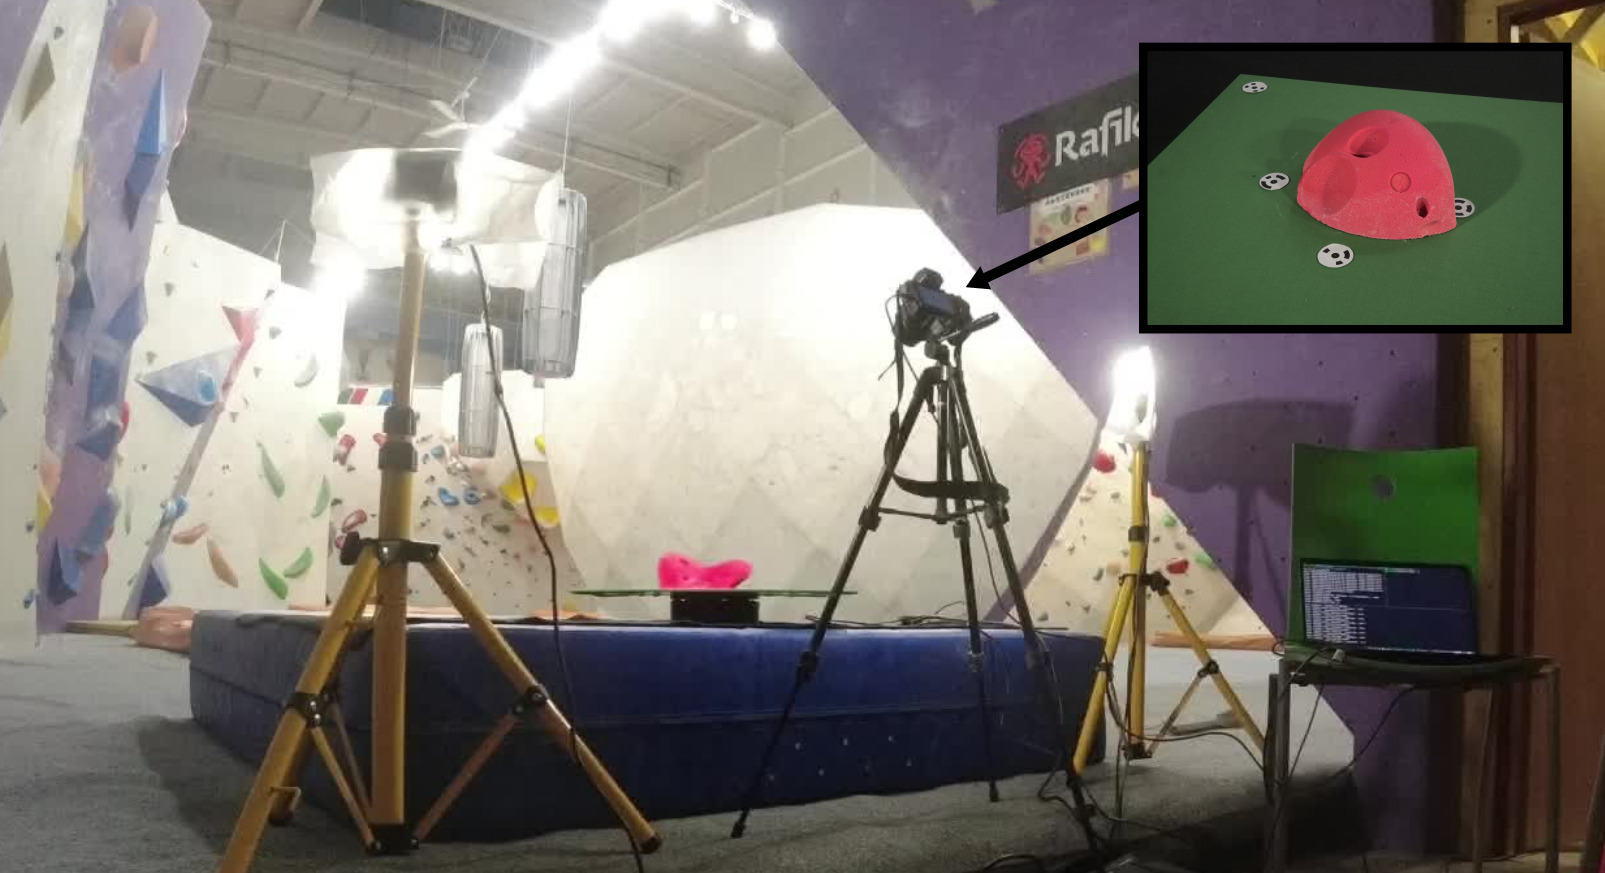
\includegraphics[width=\columnwidth]{images/setup/setup.png}
	\caption{An image of the setup during scanning, including the taken image.}
\end{figure}

\subsection{Dual texture holds}
Glossy surfaces are one of the most problematic types surfaces for photogrammetry, since the angle under which they are imaged change their appearance due to light reflecting into the camera.
This poses a problem for „dual-texture“ holds which, as the name suggests, contain two textures -- a mate texture that is meant for the climber to hold (or step) onto, and the glossy texture which is usually not.
They are increasingly used in modern bouldering and sports climbing, because they give setters more freedom in creating difficult routes.

A standard way of dealing with glossy surfaces is to cover them in something that is mate.
While this does solve the problem of model generation, it ruins the texture, because the mate solution is usually opaque (and possibly requiring another set of images for texturing).

In our case, however, the solution is rather obvious -- cover them in climbing chalk (figure \ref{fig:chalk}).
Since it is mate, it reduces the reflections of the glossy surface and provides additional feature points, making it easier for the photogrammetry software to reconstruct the model.
Additionally, since climbing chalk will be applied to the holds by climber during regular usage anyway, there is no need to obtain more images for texturing.

\begin{figure}
	\centering
	\subfloat[\centering]{{\includegraphics[height=2.5cm]{images/holds/1.png} }}%
	\hfill
	\subfloat[\centering]{{\includegraphics[height=2.5cm]{images/holds/2.png} }}%
	\hfill
	\subfloat[\centering]{{\includegraphics[height=2.5cm]{images/holds/3.png} }}%
	\caption{Example of holds with chalk applied. Some reflections are still visible, but they are not as pronounced as with no chalk applied.}%
	\label{fig:chalk}
\end{figure}

\section{Editor implementation}
The editor has been created using the Unity editor, with the majority of the codebase being written in C\#.
Besides the builtin libraries, a number of freely available user packages were used for simplifying the coding process, namely

\begin{itemize}
	\item \textbf{Quick Outline} \footnote{\url{https://assetstore.unity.com/packages/tools/particles-effects/quick-outline-115488}} -- object outline creator (for hold highlights).
	\item \textbf{OBJImport} \footnote{\url{https://assetstore.unity.com/packages/tools/modeling/runtime-obj-importer-49547}} -- an \verb|.obj| file importer (including texture files).
	\item \textbf{StandaloneFileBrowser} \footnote{\url{https://github.com/gkngkc/UnityStandaloneFileBrowser}} -- a cross-platform file browser.
\end{itemize}

The editor is cross-platform and can be run on Mac, Windows and Linux, with the newest builds being freely available at the project GitHub page \footnote{\url{https://github.com/Climber-Tools/Cled}}.

\subsection{Modes}
The editor contains three modes in which 

\subsection{Hold picking}
Picking which holds to place on the wall quickly is crucial for effective virtual route setting.
The editor contains a hold picking menu from which a subset of holds can be selected and cycled while editing.
Filtering holds can be done by selecting a specific hold color, type, manufacturer, or custom hold label.
Additionally, hovering on each of the holds rotates them around, which is useful when the static hold image isn't descriptive enough.

TODO: obrázek toho vybírání


\subsection{Import and Export}
The import and export format for the project files is a human-readable \verb|yaml| file containing information about the state of the holds, routes, paths to the models and other metadata.
Here is an example of one such file:

TODO: příklad souboru

\subsection{Capturing images}

